\documentclass{article}
\usepackage{hyperref}
\usepackage{amsmath} % or simply amstext
\newcommand{\angstrom}{\textup{\AA}}

\title{Physical Chemistry Problems and Why We Care}
\usepackage{Sweave}
\begin{document}
\Sconcordance{concordance:Chemistry1.tex:Chemistry1.Rnw:%
1 6 1 1 0 54 1 1 2 1 0 2 1 5 0 1 1 6 0 1 2 22 1 1 2 1 0 1 1 6 0 1 2 89 %
1 1 2 1 0 3 1 1 2 1 1 3 0 2 2 7 0 2 1 4 0 1 2 18 1 1 2 1 0 2 1 6 0 2 1 %
4 0 1 2 17 1}

\maketitle

\section{Introduction}

There are several concepts in Physical Chemistry that turn out to have wide applications and we are going to explore some of them here. 

First, we should acknowledge that the early history is filled with people who had the luxury to explore rather esoteric topics, while we might be learning these as a matter of our own 'development' and with a sense of what for!  I'll try to make an argument that this stuff really does matter, but for now, let's start the problem set!


\section{Problem \#2}

In this problem we are trying to determine (caculate)...

using this site: \url{http://chem.libretexts.org/Core/Physical_and_Theoretical_Chemistry/Quantum_Mechanics/02._Fundamental_Concepts_of_Quantum_Mechanics/De_Broglie_Wavelength}

\begin{equation}
\mu = \sqrt{(3k_bT/m)}
\end{equation}


\begin{Schunk}
\begin{Sinput}
> lamdba = 2500
\end{Sinput}
\end{Schunk}

\section{On Plank's Constant}

\url{https://en.wikipedia.org/wiki/Planck_constant}



$\lambda/\angstrom$ is in the units of wavelenth per meter or meter/second/meter thus we are left with a time unit! Neat. I am not sure why they can tell us that!  Whatever...

$V_s/V$ so velocity of something over another velocity. Okay, this seems werid -- what is the s?

Finally, the hint is anything but a real hint -- basically driving more questions that it answers. 

The equation given is 

\begin{equation}
KE = EV_s
\end{equation}

\noindent where KE is kenetic energy (units?) and E is the charge of an electron (volts) and $V_s$ is velocity of ??.


We can use the photo-electric equation,

\begin{equation}
E = h\nu
\end{equation}

\begin{Schunk}
\begin{Sinput}
> one=c(2536, 2830, 3039, 3302, 3663, 4358)
> two=c(2.6, 2.11, 1.81, 1.47, 1.1, .57)
> coef(lm(one~two))
\end{Sinput}
\begin{Soutput}
(Intercept)         two 
  4713.1565   -885.1904 
\end{Soutput}
\begin{Sinput}
> plot(one,two)
\end{Sinput}
\end{Schunk}
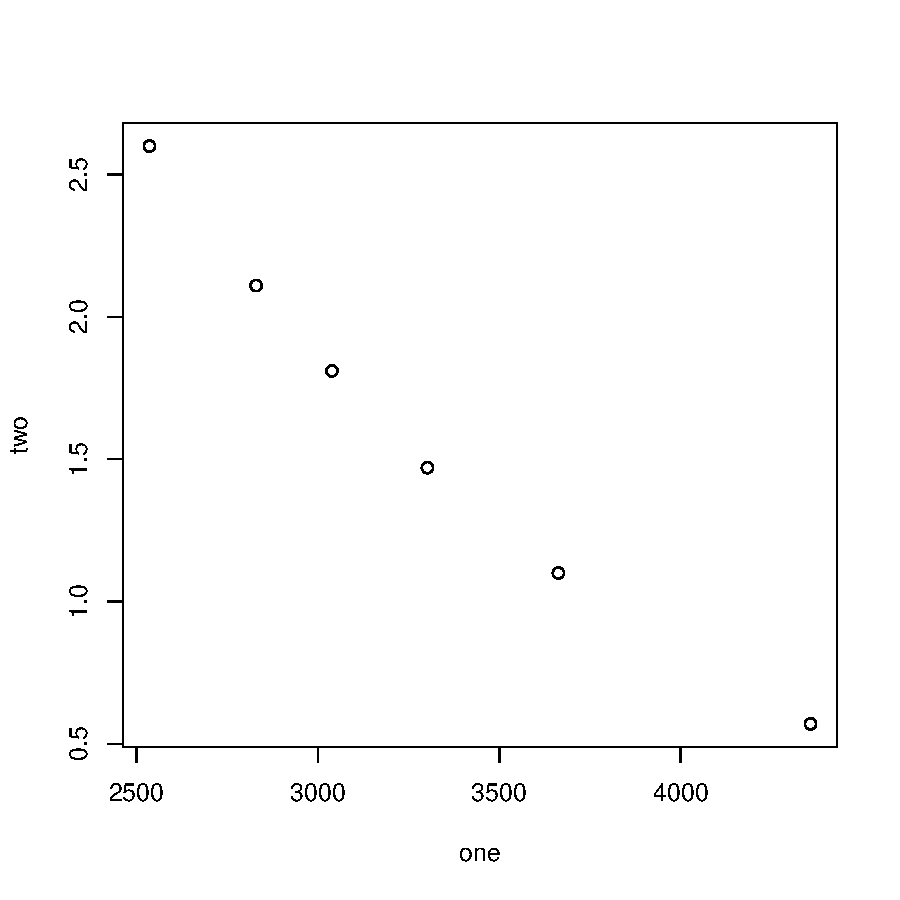
\includegraphics{Chemistry1-002}

\end{document}
